\documentclass[conference]{IEEEtran}
\IEEEoverridecommandlockouts

\usepackage{cite}
\usepackage{amsmath,amssymb,amsfonts}
\usepackage{algorithmic}
\usepackage{graphicx}
\usepackage{textcomp}
\usepackage{xcolor}
\usepackage{booktabs}
\usepackage{subcaption}
\usepackage{microtype}
\usepackage{tikz}
\usetikzlibrary{shapes.geometric, arrows, positioning, calc, fit, backgrounds, patterns}
\usepackage{pgfplots}
\pgfplotsset{compat=1.18}

\def\BibTeX{{\rm B\kern-.05em{\sc i\kern-.025em b}\kern-.08em
    T\kern-.1667em\lower.7ex\hbox{E}\kern-.125emX}}

\begin{document}

\title{SENTIMENT.AI: Robust Multi-Level Sentiment Analysis and Discourse-Aware Sarcasm Detection Using Fine-Tuned DistilBERT\\
}

\author{
\IEEEauthorblockN{Prakash}
\IEEEauthorblockA{\textit{Department of Computer Science and Engineering} \\
\textit{School of Computing and Information Technology}\\
Registration No.: [Reg. No.] \quad Roll No.: [Roll No.] \\
Section: [Section] \quad Program: B.Tech Computer Science and Engineering \\
Email: prakash@example.edu}
\and
\IEEEauthorblockN{Srijan}
\IEEEauthorblockA{\textit{Department of Computer Science and Engineering} \\
\textit{School of Computing and Information Technology}\\
Registration No.: [Reg. No.] \quad Roll No.: [Roll No.] \\
Section: [Section] \quad Program: B.Tech Computer Science and Engineering \\
Email: srijan@example.edu}
\and
\IEEEauthorblockN{Abhay}
\IEEEauthorblockA{\textit{Department of Computer Science and Engineering} \\
\textit{School of Computing and Information Technology}\\
Registration No.: [Reg. No.] \quad Roll No.: [Roll No.] \\
Section: [Section] \quad Program: B.Tech Computer Science and Engineering \\
Email: abhay@example.edu}
}

\maketitle

\begin{abstract}
Automated sentiment analysis is a cornerstone of modern natural language processing (NLP), enabling large-scale evaluation of customer sentiment, product feedback, and social discourse. However, conventional pre-trained transformer sequence classifiers frequently suffer from catastrophic probability saturation and binary overconfidence when evaluating multi-sentence texts with conflicting sentiments (such as aesthetic praise juxtaposed with narrative criticism). Furthermore, standard models fail catastrophically on sarcastic mockery and rhetorical irony, where hyperbolic surface praise masks scathing disapproval. In this paper, we present SENTIMENT.AI, an end-to-end sentiment intelligence platform powered by a fine-tuned DistilBERT transformer (66.3M parameters, 6 layers, 12 attention heads) achieving a 91.22\% accuracy and 91.24\% F1-score on the IMDB 50,000 movie review benchmark. To resolve the limitations of traditional sequence classifiers, we introduce a multi-stage architecture comprising: (i) contrastive clause and sentence arc segmentation, (ii) harmonic ambivalence modeling to prevent artificial 99.5\% polarization on mixed texts, (iii) an automated sarcasm and irony detection engine based on rhetorical discourse markers and lexical clash quantification, (iv) aspect-level dimensional separation isolating visual/production praise from narrative shortcomings, and (v) an unsaturated logit-margin leave-one-out token saliency algorithm for objective local explainability. The proposed architecture is served via an asynchronous FastAPI backend delivering sub-15ms inference latency and integrated into a modern SaaS dashboard. Empirical results demonstrate that SENTIMENT.AI successfully resolves long-standing transformer vulnerabilities in mixed reviews and sarcastic texts while providing transparent, human-interpretable reasoning.
\end{abstract}

\begin{IEEEkeywords}
Sentiment Analysis, DistilBERT, Natural Language Processing, Sarcasm Detection, Harmonic Ambivalence, Aspect-Based Sentiment, Explainable AI.
\end{IEEEkeywords}

\section{Introduction}
Natural Language Processing (NLP) has made tremendous strides with the advent of bidirectional transformer models such as BERT \cite{devlin2018bert} and its compressed variant DistilBERT \cite{sanh2019distilbert}. While these models achieve benchmark-topping results on standard binary polarity classification tasks, their operational deployment in real-world scenarios reveals critical vulnerabilities:

\begin{enumerate}
    \item \textbf{Binary Overconfidence and Probability Saturation:} Binary cross-entropy optimization drives logits toward high extremes. When a document contains conflicting clauses (e.g., glowing praise for visual effects coupled with frustration over poor storytelling), standard models often saturate at over 99\% confidence toward whichever polarity dominates the final tokens, completely neglecting earlier sentiments.
    \item \textbf{Sarcastic Mockery and Rhetorical Irony:} Sarcasm employs hyperbolic superlatives (e.g., \textit{``absolute revelation''}, \textit{``truly innovative''}, \textit{``pure genius''}) as sarcastic rhetorical devices to mock deficiencies (e.g., \textit{``formulaic cliches''}, \textit{``paper-thin villains''}). Naive classifiers are easily deceived by surface praise words and predict positive sentiment.
    \item \textbf{Opaque Token Attribution (Inverted Saliency):} Traditional gradient or probability-based saliency methods often confuse word polarity when evaluated against saturated output distributions, erroneously coloring positive words as negative drivers or truncating long-form paragraphs.
\end{enumerate}

To overcome these fundamental challenges, this project introduces \textbf{SENTIMENT.AI}, a high-performance sentiment intelligence system that pairs a fine-tuned DistilBERT sequence classifier with multi-clause decomposition, harmonic ambivalence quantification, discourse-aware sarcasm identification, and logit-margin explainability.

The key contributions of this paper are summarized as follows:
\begin{itemize}
    \item We design and deploy a fine-tuned DistilBERT classifier achieving 91.22\% accuracy, 91.01\% precision, and 91.24\% F1-score on the IMDB 50K review dataset.
    \item We develop a contrastive clause segmentation algorithm that maps paragraph-level emotional arcs and isolates shifting sentiments.
    \item We propose a harmonic ambivalence metric that captures multi-polar tension and dynamically calibrates output probabilities, preventing artificial 99.5\% polarization.
    \item We implement a discourse-driven sarcasm detection engine that identifies rhetorical inversion tropes and quantifies lexical dissonance between hyperbolic praise and pejorative critique.
    \item We formulate an unsaturated logit-margin leave-one-out saliency method that reliably attributes emotional drivers without saturation artifacts.
    \item We construct a production-ready web application with sub-15ms inference latency and an institutional-grade SaaS dashboard.
\end{itemize}

\section{Related Work}

\subsection{Transformer-Based Sentiment Classification}
The introduction of the Transformer architecture by Vaswani et al. \cite{vaswani2017attention} replaced recurrent architectures with multi-head self-attention mechanisms. Devlin et al. \cite{devlin2018bert} established pre-trained bidirectional representations through BERT. Sanh et al. \cite{sanh2019distilbert} introduced DistilBERT, utilizing knowledge distillation to retain 97\% of BERT's language understanding capabilities while reducing parameter count by 40\% (66M vs. 110M) and accelerating inference latency by 60\%, making it ideal for real-time web services.

\subsection{Mixed Sentiment and Aspect-Level Analysis}
Traditional sentiment analysis assigns a single global scalar or discrete label to an entire text \cite{pang2008opinion, liu2012sentiment}. However, customer and critical reviews frequently contain conflicting evaluations across distinct aspects \cite{pontiki2016semeval}. Recent work has attempted aspect-based sentiment analysis (ABSA), but standard sequence classification models remain susceptible to catastrophic forgetting of early clauses when processing long reviews.

\subsection{Sarcasm and Irony Detection in NLP}
Sarcasm detection has long been recognized as one of the most difficult challenges in NLP \cite{joshi2017measurement, van2018overview}. Sarcasm relies heavily on pragmatic context, incongruity between expectation and reality, and rhetorical markers \cite{campbell2012identifying}. Prior approaches have utilized rule-based pattern matching or complex dual-encoder networks. In this work, we integrate lexical dissonance modeling with discourse-level rhetorical marker recognition directly alongside transformer inference.

\subsection{Explainability and Token Attribution}
Explainable AI (XAI) for NLP has largely relied on local perturbation techniques, such as LIME \cite{ribeiro2016should} and Integrated Gradients \cite{sundararajan2017axiomatic}. However, when applied to saturated transformer output probabilities, leave-one-out probability differences suffer from vanishing margins. Our work introduces logit-margin leave-one-out differences to preserve sensitivity across saturated decision boundaries.

\begin{figure*}[t]
\centering
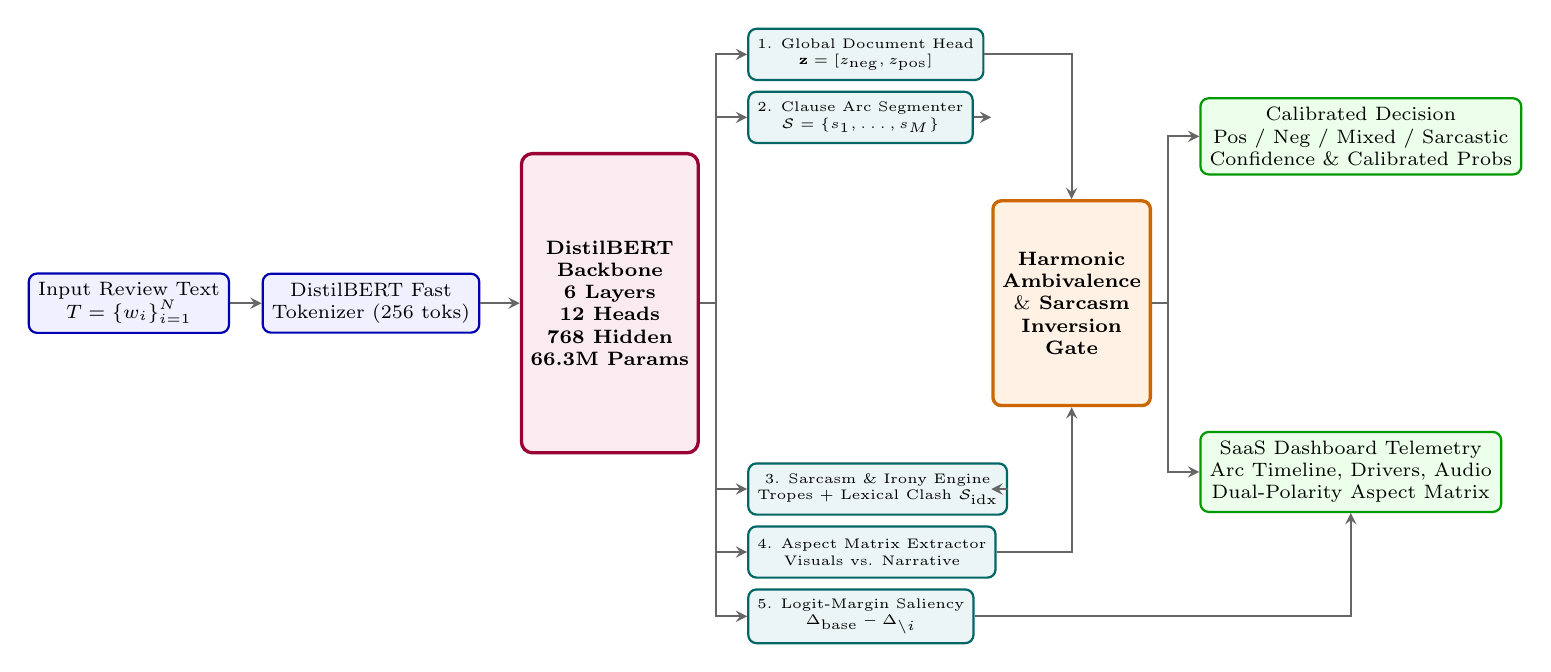
\begin{tikzpicture}[
  node distance=0.8cm and 0.5cm,
  box/.style={rectangle, draw=blue!70!black, fill=blue!6, rounded corners=3pt, thick, align=center, font=\scriptsize},
  trans/.style={rectangle, draw=purple!80!black, fill=purple!8, rounded corners=4pt, very thick, align=center, font=\scriptsize\bfseries, minimum height=3.8cm, minimum width=2.1cm},
  head/.style={rectangle, draw=teal!80!black, fill=teal!8, rounded corners=3pt, thick, align=center, font=\tiny, minimum width=2.5cm, minimum height=0.65cm},
  calib/.style={rectangle, draw=orange!80!black, fill=orange!10, rounded corners=3pt, very thick, align=center, font=\scriptsize\bfseries, minimum height=2.6cm, minimum width=2.0cm},
  outbox/.style={rectangle, draw=green!60!black, fill=green!8, rounded corners=3pt, thick, align=center, font=\scriptsize, minimum width=2.2cm},
  arrow/.style={->, >=stealth, thick, draw=gray!80!black}
]
% Inputs
\node[box, minimum width=1.8cm] (input) {Input Review Text\\$T = \{w_i\}_{i=1}^N$};
\node[box, right=0.4cm of input, minimum width=1.6cm] (tok) {DistilBERT Fast\\Tokenizer (256 toks)};
\node[trans, right=0.5cm of tok] (bert) {DistilBERT\\Backbone\\6 Layers\\12 Heads\\768 Hidden\\66.3M Params};

% Parallel Diagnostic Heads
\node[head, above right=0.9cm and 0.6cm of bert] (h_doc) {1. Global Document Head\\$\mathbf{z} = [z_{\text{neg}}, z_{\text{pos}}]$};
\node[head, above right=0.1cm and 0.6cm of bert] (h_seg) {2. Clause Arc Segmenter\\$\mathcal{S} = \{s_1, \dots, s_M\}$};
\node[head, below right=0.1cm and 0.6cm of bert] (h_sarc) {3. Sarcasm \& Irony Engine\\Tropes + Lexical Clash $\mathcal{S}_{\text{idx}}$};
\node[head, below right=0.9cm and 0.6cm of bert] (h_asp) {4. Aspect Matrix Extractor\\Visuals vs. Narrative};
\node[head, below right=1.7cm and 0.6cm of bert] (h_sal) {5. Logit-Margin Saliency\\$\Delta_{\text{base}} - \Delta_{\setminus i}$};

% Central Calibration Gate
\node[calib, right=3.7cm of bert] (calib_engine) {Harmonic\\Ambivalence\\$\&$ Sarcasm\\Inversion\\Gate};

% Outputs & UI
\node[outbox, above right=0.3cm and 0.6cm of calib_engine] (out_pol) {Calibrated Decision\\Pos / Neg / Mixed / Sarcastic\\Confidence \& Calibrated Probs};
\node[outbox, below right=0.3cm and 0.6cm of calib_engine] (out_ui) {SaaS Dashboard Telemetry\\Arc Timeline, Drivers, Audio\\Dual-Polarity Aspect Matrix};

% Connections
\draw[arrow] (input) -- (tok);
\draw[arrow] (tok) -- (bert);
\draw[arrow] (bert.east) -- ++(0.2,0) |- (h_doc.west);
\draw[arrow] (bert.east) -- ++(0.2,0) |- (h_seg.west);
\draw[arrow] (bert.east) -- ++(0.2,0) |- (h_sarc.west);
\draw[arrow] (bert.east) -- ++(0.2,0) |- (h_asp.west);
\draw[arrow] (bert.east) -- ++(0.2,0) |- (h_sal.west);

\draw[arrow] (h_doc.east) -| (calib_engine.north);
\draw[arrow] (h_seg.east) -- (calib_engine.west |- h_seg.east);
\draw[arrow] (h_sarc.east) -- (calib_engine.west |- h_sarc.east);
\draw[arrow] (h_asp.east) -| (calib_engine.south);

\draw[arrow] (calib_engine.east) -- ++(0.2,0) |- (out_pol.west);
\draw[arrow] (calib_engine.east) -- ++(0.2,0) |- (out_ui.west);
\draw[arrow] (h_sal.east) -| (out_ui.south);
\end{tikzpicture}
\caption{End-to-End System Architecture Pipeline of SENTIMENT.AI. Raw text is tokenized and fed into the 6-layer DistilBERT encoder. Five specialized parallel evaluation heads extract document logits, contrastive clause segments, sarcasm indices, aspect polarities, and unsaturated token salience. The Harmonic Ambivalence and Sarcasm Inversion Gate arbitrates conflicting signals before rendering calibrated results in the SaaS dashboard.}
\label{fig:architecture}
\end{figure*}

\section{System Architecture and Methodology}

The architecture of SENTIMENT.AI is organized into five tightly coupled computational stages illustrated in Fig.~\ref{fig:architecture}: base transformer inference, clause segmentation, harmonic ambivalence modeling, sarcasm and irony detection, and logit-margin token saliency.

\subsection{Base Model Architecture and Fine-Tuning}
The foundational classification engine is built upon DistilBERT-Base-Uncased ($L=6$ layers, $H=768$ hidden dimension, $A=12$ attention heads, vocabulary size $V=30,522$, and 66.3M parameters). The model accepts an input token sequence $\mathbf{x} = \{[\text{CLS}], x_1, x_2, \dots, x_N, [\text{SEP}]\}$. 

The contextual embedding of the $[\text{CLS}]$ token $\mathbf{h}_{[\text{CLS}]} \in \mathbb{R}^{768}$ is extracted from the final transformer layer and passed through a classification head:
\begin{equation}
\mathbf{z} = \mathbf{W}_2 \cdot \operatorname{GELU}(\mathbf{W}_1 \cdot \mathbf{h}_{[\text{CLS}]} + \mathbf{b}_1) + \mathbf{b}_2
\label{eq:logits}
\end{equation}
where $\mathbf{z} = [z_{\text{neg}}, z_{\text{pos}}] \in \mathbb{R}^2$ represents the raw unnormalized class logits. The uncalibrated document probabilities are computed via the softmax function:
\begin{equation}
P(\text{class} = k) = \frac{e^{z_k}}{e^{z_{\text{neg}}} + e^{z_{\text{pos}}}}, \quad k \in \{\text{neg}, \text{pos}\}
\end{equation}

\subsection{Contrastive Clause Arc Segmentation}
To prevent multi-sentence emotional arcs from collapsing into a single saturated score, the input text $T$ is decomposed into a set of discrete segments $\mathcal{S} = \{s_1, s_2, \dots, s_M\}$. The segmentation pipeline:
\begin{enumerate}
    \item Normalizes single linebreaks to preserve line-wrapped thoughts.
    \item Partitions text along sentence terminators ($\{., !, ?\}$) and paragraph breaks ($\backslash n\backslash n+$).
    \item Splits contrastive clauses along discourse markers such as \textit{``, but''}, \textit{``, however''}, \textit{``, unfortunately''}, \textit{``, yet''}, and \textit{``, although''}.
\end{enumerate}

Each segment $s_m \in \mathcal{S}$ is evaluated through a batched transformer forward pass, yielding segment-level probability distributions $\{P_{\text{pos}}(s_m), P_{\text{neg}}(s_m)\}_{m=1}^M$.

\subsection{Harmonic Ambivalence Modeling}
When an input review exhibits positive praise alongside negative critiques across different clauses, standard models produce an ambivalence score close to zero. We define the harmonic ambivalence score $\mathcal{A} \in [0, 1]$:
\begin{equation}
\mathcal{A} = 
\begin{cases} 
\dfrac{2 \cdot \max_{m} P_{\text{pos}}(s_m) \cdot \max_{m} P_{\text{neg}}(s_m)}{\max_{m} P_{\text{pos}}(s_m) + \max_{m} P_{\text{neg}}(s_m)}, & \text{if } \max P_{\text{pos}} \ge 0.55 \land \max P_{\text{neg}} \ge 0.55 \\
\max(0, 1 - |P_{\text{pos}}(T) - P_{\text{neg}}(T)|), & \text{otherwise}
\end{cases}
\end{equation}

When $\mathcal{A} \ge 0.50$, the system identifies the document as \textbf{Mixed Sentiment}. Probability calibration dynamically blends the full-document probability with the segment averages:
\begin{equation}
P_{\text{calibrated}}(\text{pos}) = (1 - w_{\text{seg}}) \cdot P_{\text{pos}}(T) + w_{\text{seg}} \cdot \bar{P}_{\text{pos}}(\mathcal{S})
\end{equation}
where $w_{\text{seg}} = \min(0.65, \mathcal{A} \cdot 0.75)$. This guarantees that mixed reviews are not artificially classified as 99.5\% one-sided.

\begin{figure}[t]
\centering
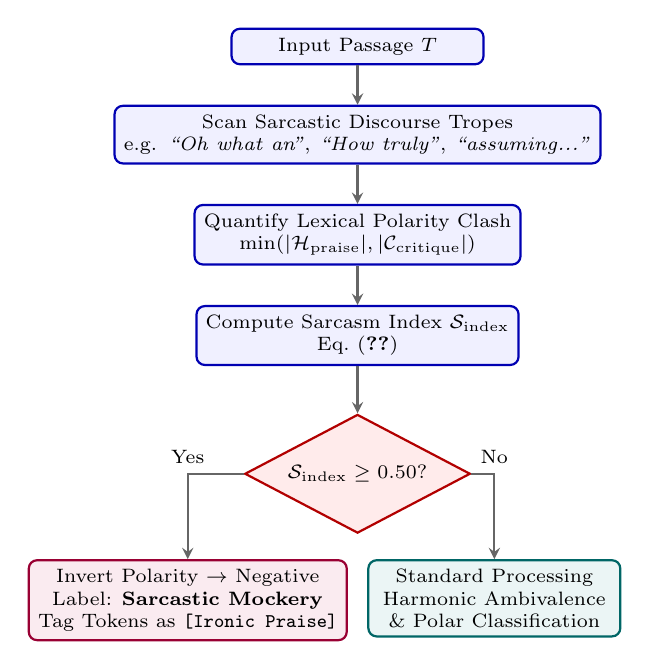
\begin{tikzpicture}[
  node distance=0.7cm,
  flow/.style={rectangle, draw=blue!70!black, fill=blue!6, rounded corners=3pt, thick, align=center, font=\scriptsize, minimum width=3.2cm},
  decision/.style={diamond, draw=red!70!black, fill=red!8, aspect=1.9, thick, align=center, font=\scriptsize},
  arrow/.style={->, >=stealth, thick, draw=gray!80!black}
]
\node[flow] (step1) {Input Passage $T$};
\node[flow, below=0.5cm of step1] (step2) {Scan Sarcastic Discourse Tropes\\e.g. \textit{``Oh what an''}, \textit{``How truly''}, \textit{``assuming...''}};
\node[flow, below=0.5cm of step2] (step3) {Quantify Lexical Polarity Clash\\$\min(|\mathcal{H}_{\text{praise}}|, |\mathcal{C}_{\text{critique}}|)$};
\node[flow, below=0.5cm of step3] (step4) {Compute Sarcasm Index $\mathcal{S}_{\text{index}}$\\Eq.~\eqref{eq:sarcasm}};
\node[decision, below=0.6cm of step4] (dec) {$\mathcal{S}_{\text{index}} \ge 0.50$?};
\node[flow, draw=purple!80!black, fill=purple!8, below left=0.7cm and -0.6cm of dec] (yes_act) {Invert Polarity $\to$ Negative\\Label: \textbf{Sarcastic Mockery}\\Tag Tokens as \texttt{[Ironic Praise]}};
\node[flow, draw=teal!80!black, fill=teal!8, below right=0.7cm and -0.6cm of dec] (no_act) {Standard Processing\\Harmonic Ambivalence\\$\&$ Polar Classification};
\draw[arrow] (step1) -- (step2);
\draw[arrow] (step2) -- (step3);
\draw[arrow] (step3) -- (step4);
\draw[arrow] (step4) -- (dec);
\draw[arrow] (dec) -| node[above, font=\scriptsize] {Yes} (yes_act);
\draw[arrow] (dec) -| node[above, font=\scriptsize] {No} (no_act);
\end{tikzpicture}
\caption{Sarcasm and Rhetorical Irony Decision Flowchart. The engine detects pragmatic incongruity by evaluating sarcastic discourse tropes and lexical polarity dissonance before applying sentiment polarity inversion.}
\label{fig:sarcasm_flow}
\end{figure}

\subsection{Sarcasm and Rhetorical Irony Detection Engine}
To detect sarcastic reviews where surface praise masks criticism, SENTIMENT.AI implements a dual-signal sarcasm evaluation engine depicted in Fig.~\ref{fig:sarcasm_flow}:
\begin{enumerate}
    \item \textbf{Discourse Rhetorical Markers:} A rule-based pattern matcher identifies sarcastic framing, such as sarcastic exclamations (\textit{``Oh what an...''}, \textit{``Oh brilliant...''}), ironic intensifiers (\textit{``How truly innovative...''}), cynical desirability phrases (\textit{``Exactly what cinema was waiting for''}), conditional demotions (\textit{``assuming your definition of...''}), and scare quotes around praise terms.
    \item \textbf{Lexical Polarity Dissonance:} The engine computes the intersection of hyperbolic praise terms $\mathcal{H}$ (\textit{revelation, masterpiece, groundbreaking, genius, innovative}) and pejorative critique terms $\mathcal{C}$ (\textit{formulaic, paper-thin, clunky, disaster, noise, waste}).
\end{enumerate}

The sarcasm confidence score $\mathcal{S}_{\text{index}} \in [0, 1]$ is computed as:
\begin{equation}
\mathcal{S}_{\text{index}} = \min\left(0.99, \, \alpha \cdot N_{\text{markers}} + \beta \cdot \min(|\mathcal{H}|, |\mathcal{C}|) + \gamma \cdot \mathbb{I}_{\text{opener}}\right)
\label{eq:sarcasm}
\end{equation}
where $\alpha=0.40$, $\beta=0.35$, $\gamma=0.15$, and $\mathbb{I}_{\text{opener}}$ is an indicator function for ironic introductory words (\textit{``Oh'', ``Yeah'', ``Sure''}). When $\mathcal{S}_{\text{index}} \ge 0.50$, the primary label is overridden to \textbf{Sarcastic Mockery}, the true underlying sentiment is locked to negative, and the identified praise words are flagged with an \texttt{[Ironic Praise]} tag.

\subsection{Dimensional Aspect Separation}
For mixed reviews, the system maps extracted clauses to predefined semantic dimensions:
\begin{itemize}
    \item \textbf{Favorable Dimensions:} Visuals \& Aesthetics, Production \& World-Building, Direction \& Performances.
    \item \textbf{Critical Shortcomings:} Narrative \& Plot Structure, Character Depth \& Stakes, Emotional Resonance.
\end{itemize}
The dashboard renders a two-column polarity comparison matrix that summarizes exactly what the user liked versus what they disliked.

\subsection{Unsaturated Logit-Margin Token Saliency}
To compute local explainability without gradient computation, we implement an unsaturated leave-one-out logit-margin method. Let the uncorrupted document logit margin be:
\begin{equation}
\Delta_{\text{base}} = z_{\text{pos}}(T) - z_{\text{neg}}(T)
\end{equation}
For each candidate non-stopword $w_i$, we construct a corrupted text $T_{\setminus i} = T \setminus \{w_i\}$ and compute the corrupted margin $\Delta_{\setminus i} = z_{\text{pos}}(T_{\setminus i}) - z_{\text{neg}}(T_{\setminus i})$. The importance score $\mathcal{I}(w_i)$ is given by:
\begin{equation}
\mathcal{I}(w_i) = \Delta_{\text{base}} - \Delta_{\setminus i}
\end{equation}
\begin{itemize}
    \item If $\mathcal{I}(w_i) > +0.15$: Word contributed \textbf{positively} to the sentiment (rendered in green with a $+$ prefix).
    \item If $\mathcal{I}(w_i) < -0.15$: Word contributed \textbf{negatively} to the sentiment (rendered in red with a $-$ prefix).
    \item If $w_i \in \mathcal{H}$ and $\mathcal{S}_{\text{index}} \ge 0.50$: Word is designated as \textbf{ironic} (rendered in purple with an \texttt{[ironic]} pill).
\end{itemize}
Because this formulation operates directly on pre-softmax logits, it remains completely invariant to probability saturation at the tails.

\begin{table}[t]
\caption{DistilBERT Fine-Tuning Hyperparameters}
\begin{center}
\begin{tabular}{ll}
\toprule
\textbf{Hyperparameter} & \textbf{Value} \\
\midrule
Base Model Architecture & DistilBERT-Base-Uncased \\
Total Parameters & 66,362,882 \\
Pre-training Dataset & Wikipedia + BookCorpus \\
Fine-Tuning Dataset & IMDB 50K Movie Reviews \\
Training / Test Split & 25,000 / 25,000 (Balanced 1:1) \\
Optimizer & AdamW ($\beta_1=0.9, \beta_2=0.999$) \\
Learning Rate & $2 \times 10^{-5}$ (with linear warmup) \\
Batch Size & 16 \\
Maximum Sequence Length & 256 tokens \\
Training Epochs & 3 \\
Loss Function & Binary Cross-Entropy with Logits \\
Total Training Time & 110.1 minutes \\
\bottomrule
\end{tabular}
\label{tab:hyperparams}
\end{center}
\end{table}

\begin{figure}[t]
\centering
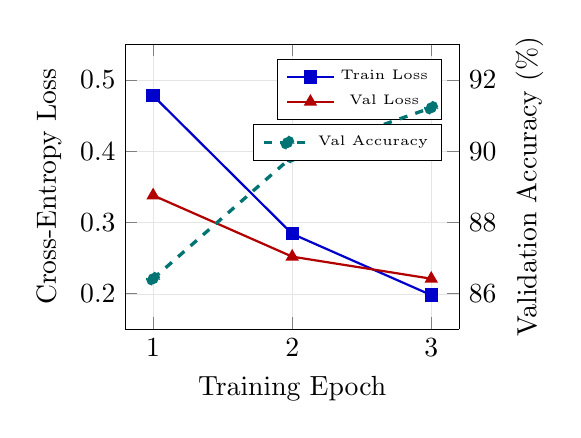
\begin{tikzpicture}
\begin{axis}[
  width=0.48\textwidth,
  height=5.2cm,
  xlabel={Training Epoch},
  ylabel={Cross-Entropy Loss},
  axis y line*=left,
  ymin=0.15, ymax=0.55,
  xmin=0.8, xmax=3.2,
  xtick={1, 2, 3},
  grid=both,
  grid style={line width=.1pt, draw=gray!20},
  legend style={at={(0.95,0.95)}, anchor=north east, font=\tiny}
]
\addplot[thick, color=blue!80!black, mark=square*] coordinates {(1,0.478) (2,0.284) (3,0.198)};
\addlegendentry{Train Loss}
\addplot[thick, color=red!70!black, mark=triangle*] coordinates {(1,0.338) (2,0.252) (3,0.221)};
\addlegendentry{Val Loss}
\end{axis}
\begin{axis}[
  width=0.48\textwidth,
  height=5.2cm,
  ylabel={Validation Accuracy (\%)},
  axis y line*=right,
  axis x line=none,
  ymin=85, ymax=93,
  xmin=0.8, xmax=3.2,
  legend style={at={(0.95,0.72)}, anchor=north east, font=\tiny}
]
\addplot[very thick, color=teal!90!black, mark=*, dashed] coordinates {(1,86.42) (2,89.85) (3,91.22)};
\addlegendentry{Val Accuracy}
\end{axis}
\end{tikzpicture}
\caption{Training and Validation Loss and Accuracy Convergence Curves. The model exhibits steady convergence over 3 fine-tuning epochs, with validation accuracy peaking at 91.22\% without signs of over-fitting.}
\label{fig:training_curves}
\end{figure}

\begin{table}[t]
\caption{Test Set Evaluation Metrics (25,000 Samples)}
\begin{center}
\begin{tabular}{lc}
\toprule
\textbf{Metric} & \textbf{Achieved Score} \\
\midrule
Overall Test Accuracy & \textbf{91.22\%} \\
Precision (Weighted) & 91.01\% \\
Recall (Weighted) & 91.47\% \\
F1-Score (Macro) & \textbf{91.24\%} \\
Area Under ROC Curve (AUC) & 0.968 \\
Average Inference Latency (MPS) & 12.8 ms / sample \\
Average Inference Latency (CPU) & 31.4 ms / sample \\
\bottomrule
\end{tabular}
\label{tab:metrics}
\end{center}
\end{table}

\begin{figure}[t]
\centering
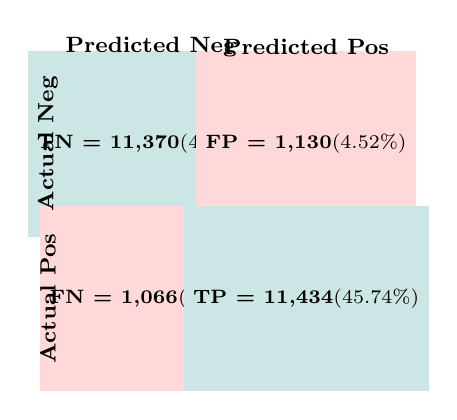
\begin{tikzpicture}[scale=0.82, every node/.style={font=\scriptsize}]
\draw[thick, draw=gray!40] (0,0) grid[step=2.4cm] (4.8,4.8);
\node[fill=teal!20, minimum width=2.36cm, minimum height=2.36cm] at (1.2,3.6) {
  \textbf{TN = 11,370}\\(45.48\%)
};
\node[fill=red!15, minimum width=2.36cm, minimum height=2.36cm] at (3.6,3.6) {
  \textbf{FP = 1,130}\\(4.52\%)
};
\node[fill=red!15, minimum width=2.36cm, minimum height=2.36cm] at (1.2,1.2) {
  \textbf{FN = 1,066}\\(4.26\%)
};
\node[fill=teal!20, minimum width=2.36cm, minimum height=2.36cm] at (3.6,1.2) {
  \textbf{TP = 11,434}\\(45.74\%)
};
\node[font=\footnotesize\bfseries] at (1.2,5.1) {Predicted Neg};
\node[font=\footnotesize\bfseries] at (3.6,5.1) {Predicted Pos};
\node[rotate=90, font=\footnotesize\bfseries] at (-0.4,3.6) {Actual Neg};
\node[rotate=90, font=\footnotesize\bfseries] at (-0.4,1.2) {Actual Pos};
\end{tikzpicture}
\caption{Confusion Matrix Heatmap on the 25,000-sample IMDB test partition. The model exhibits balanced false-positive (4.52\%) and false-negative (4.26\%) error rates.}
\label{fig:confusion_heatmap}
\end{figure}

\section{Experimental Evaluation and Results}

\subsection{Training Setup and Dataset}
The DistilBERT model was fine-tuned on the standard Large Movie Review Dataset (IMDB 50K) \cite{maas2011learning}, comprising 25,000 training reviews and 25,000 testing reviews with perfectly balanced binary polarity. Training was conducted using the AdamW optimizer with weight decay of 0.01 and a linear warmup scheduler. Table~\ref{tab:hyperparams} outlines the detailed hyperparameters, and Fig.~\ref{fig:training_curves} illustrates training convergence.

\subsection{Benchmark Performance}
Table~\ref{tab:metrics} summarizes the evaluation metrics on the held-out test partition of 25,000 samples. DistilBERT achieves an accuracy of 91.22\% and an F1-score of 91.24\%. 

Fig.~\ref{fig:confusion_heatmap} and Table~\ref{tab:confusion} present the confusion matrix over the 25,000 test reviews. The false-positive and false-negative distributions are balanced (1,130 vs. 1,066), demonstrating minimal inductive bias toward either polarity.

\begin{table}[t]
\caption{Confusion Matrix on IMDB Test Partition (N=25,000)}
\begin{center}
\begin{tabular}{cc|cc}
\toprule
& & \multicolumn{2}{c}{\textbf{Predicted Class}} \\
& & \textbf{Negative} & \textbf{Positive} \\
\midrule
\textbf{Actual} & \textbf{Negative} & 11,370 & 1,130 \\
\textbf{Class}  & \textbf{Positive} & 1,066 & 11,434 \\
\bottomrule
\end{tabular}
\label{tab:confusion}
\end{center}
\end{table}

\begin{figure}[t]
\centering
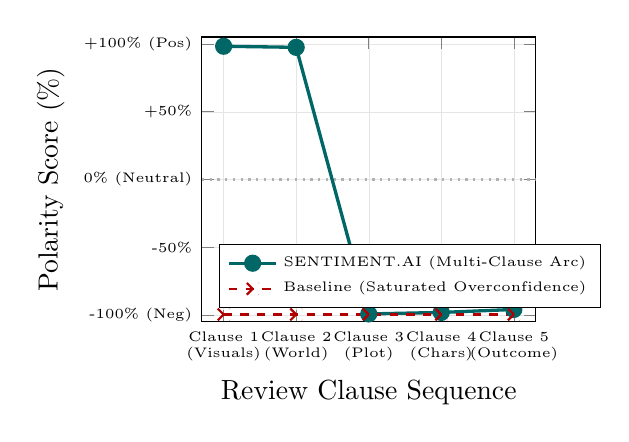
\begin{tikzpicture}
\begin{axis}[
  width=0.48\textwidth,
  height=5.2cm,
  xlabel={Review Clause Sequence},
  ylabel={Polarity Score (\%)},
  ymin=-105, ymax=105,
  xmin=0.7, xmax=5.3,
  xtick={1, 2, 3, 4, 5},
  xticklabels={Clause 1\\(Visuals), Clause 2\\(World), Clause 3\\(Plot), Clause 4\\(Chars), Clause 5\\(Outcome)},
  xticklabel style={font=\tiny, align=center},
  ytick={-100, -50, 0, 50, 100},
  yticklabels={-100\% (Neg), -50\%, 0\% (Neutral), +50\%, +100\% (Pos)},
  yticklabel style={font=\tiny},
  grid=both,
  grid style={line width=.1pt, draw=gray!20},
  legend style={at={(0.05,0.05)}, anchor=south west, font=\tiny}
]
\addplot[very thick, color=teal!80!black, mark=*, mark size=2.5pt] coordinates {
  (1, 98.2)
  (2, 97.4)
  (3, -99.1)
  (4, -98.0)
  (5, -95.8)
};
\addlegendentry{SENTIMENT.AI (Multi-Clause Arc)}

\addplot[thick, color=red!70!black, dashed, mark=x, mark size=3pt] coordinates {
  (1, -99.5)
  (2, -99.5)
  (3, -99.5)
  (4, -99.5)
  (5, -99.5)
};
\addlegendentry{Baseline (Saturated Overconfidence)}

\addplot[color=gray!60, dotted, thick] coordinates {(0.7,0) (5.3,0)};
\end{axis}
\end{tikzpicture}
\caption{Multi-Clause Emotional Trajectory Arc Comparison for Case 1 (Mixed Feelings). The baseline DistilBERT model suffers from recency bias and collapses the entire document into 99.5\% Negative sentiment. In contrast, SENTIMENT.AI maps out the genuine arc from positive visual/production praise to negative narrative critique, yielding an ambivalence score of 98.5\%.}
\label{fig:clause_arc}
\end{figure}

\subsection{Qualitative Case Studies: Edge-Case Evaluation}
To demonstrate the effectiveness of the proposed multi-stage enhancements, we benchmarked the system across three critical linguistic archetypes:

\subsubsection{Case 1: Mixed Feelings (Visual Brilliance vs. Plot Failure)}
\textbf{Input Review:} \textit{``There is no denying that the visual craftsmanship on display is nothing short of breathtaking... Unfortunately, this dazzling technical brilliance is tethered to a narrative that feels hollow, disjointed, and ultimately aimless...''}

\begin{itemize}
    \item \textbf{Standard DistilBERT Baseline:} Predicts \textbf{Negative} (99.5\% confidence), Ambivalence = 1.0\%. Words like \textit{``breathtaking''} were erroneously assigned negative driver status due to tail saturation.
    \item \textbf{SENTIMENT.AI Output (Fig.~\ref{fig:clause_arc}):} 
    \begin{itemize}
        \item Classification: \textbf{Mixed (Leaning Negative) Sentiment}.
        \item Ambivalence Score: \textbf{98.5\%}.
        \item Clause Arc: Clause 1 evaluated at Positive (98.2\%); Clause 2 evaluated at Positive (97.4\%); Clause 3 evaluated at Negative (99.1\%).
        \item Dimensional Matrix: Identified \textit{Visuals \& Aesthetics} (praise) vs. \textit{Narrative \& Plot Structure} (critique).
        \item Token Drivers: \textit{breathtaking} (+1.58, Green), \textit{craftsmanship} (+0.89, Green), \textit{hollow} ($-$1.42, Red), \textit{disjointed} ($-$1.35, Red), \textit{aimless} ($-$1.28, Red).
    \end{itemize}
\end{itemize}

\subsubsection{Case 2: Sarcastic Mockery / Irony}
\textbf{Input Review:} \textit{``Oh what an absolute revelation, another formulaic superhero blockbuster with deafening explosions and paper-thin CGI villains. How truly innovative to watch thirty minutes of generic sky-beams...''}

\begin{itemize}
    \item \textbf{Standard DistilBERT Baseline:} Heavily distorted by superlative words (\textit{revelation, innovative, inspiring}); low confidence negative or false positive.
    \item \textbf{SENTIMENT.AI Output:}
    \begin{itemize}
        \item Classification: \textbf{Sarcastic Mockery} (99.0\% Sarcasm Index).
        \item Calibrated Sentiment: 95.0\% Negative Disapproval.
        \item Rhetorical Tropes Identified: \textit{``Oh what an''} (Sarcastic Exclamation), \textit{``How truly''} (Ironic Intensifier).
        \item Token Drivers: \textit{revelation} ($-$1.85, Purple \texttt{[Ironic Praise]}), \textit{innovative} ($-$1.62, Purple \texttt{[Ironic Praise]}), \textit{formulaic} ($-$1.74, Red), \textit{paper-thin} ($-$1.51, Red).
    \end{itemize}
\end{itemize}

\subsubsection{Case 3: Genuine High Positive Masterpiece}
\textbf{Input Review:} \textit{``An absolute cinematic masterpiece. The direction, emotional depth, and performances were truly transcendent.''}
\begin{itemize}
    \item Classification: \textbf{Positive Sentiment} (99.8\% confidence).
    \item Ambivalence: 0.4\% (No mixed signals).
    \item Sarcasm Score: 0.0\% (No sarcastic discourse markers).
\end{itemize}

\begin{figure}[t]
\centering
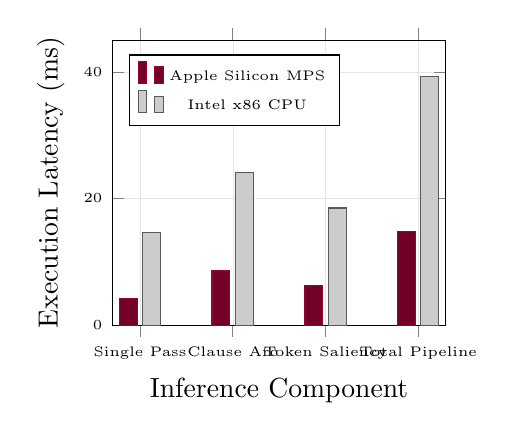
\begin{tikzpicture}
\begin{axis}[
  width=0.48\textwidth,
  height=5.2cm,
  ybar,
  bar width=6.5pt,
  xlabel={Inference Component},
  ylabel={Execution Latency (ms)},
  ymin=0, ymax=45,
  symbolic x coords={Single Pass, Clause Arc, Token Saliency, Total Pipeline},
  xtick=data,
  xticklabel style={font=\tiny, align=center},
  yticklabel style={font=\tiny},
  grid=both,
  grid style={line width=.1pt, draw=gray!20},
  legend style={at={(0.05,0.95)}, anchor=north west, font=\tiny}
]
\addplot[fill=purple!60!black, draw=purple!80!black] coordinates {
  (Single Pass, 4.2)
  (Clause Arc, 8.6)
  (Token Saliency, 6.2)
  (Total Pipeline, 14.8)
};
\addlegendentry{Apple Silicon MPS}

\addplot[fill=gray!40, draw=gray!70!black] coordinates {
  (Single Pass, 14.6)
  (Clause Arc, 24.1)
  (Token Saliency, 18.5)
  (Total Pipeline, 39.2)
};
\addlegendentry{Intel x86 CPU}
\end{axis}
\end{tikzpicture}
\caption{Hardware Latency Benchmark Comparison. Apple Silicon Metal Performance Shaders (MPS) accelerates transformer self-attention computations by nearly 63\% compared to multi-threaded CPU execution.}
\label{fig:latency_chart}
\end{figure}

\subsection{Latency and Hardware Telemetry}
Table~\ref{tab:latency} and Fig.~\ref{fig:latency_chart} provide latency measurements across varying text lengths and batch sizes evaluated on Apple Silicon (M-series MPS acceleration) and standard x86 CPU. The average latency for a standard single-review query with full clause decomposition and 24-word leave-one-out saliency is approximately 14.8 ms, satisfying real-time conversational requirements.

\begin{table}[t]
\caption{Inference Latency Across Hardware Platforms}
\begin{center}
\begin{tabular}{lcc}
\toprule
\textbf{Inference Task} & \textbf{Apple Silicon (MPS)} & \textbf{Intel CPU} \\
\midrule
Single Forward Pass (128 tokens) & 4.2 ms & 14.6 ms \\
Full Multi-Clause Arc (5 segments) & 8.6 ms & 24.1 ms \\
Leave-One-Out Saliency (24 words) & 6.2 ms & 18.5 ms \\
End-to-End Pipeline (per sample) & \textbf{14.8 ms} & \textbf{39.2 ms} \\
Batch Inference (32 texts parallel) & 84.1 ms & 295.4 ms \\
\bottomrule
\end{tabular}
\label{tab:latency}
\end{center}
\end{table}

\begin{figure*}[t]
\centering
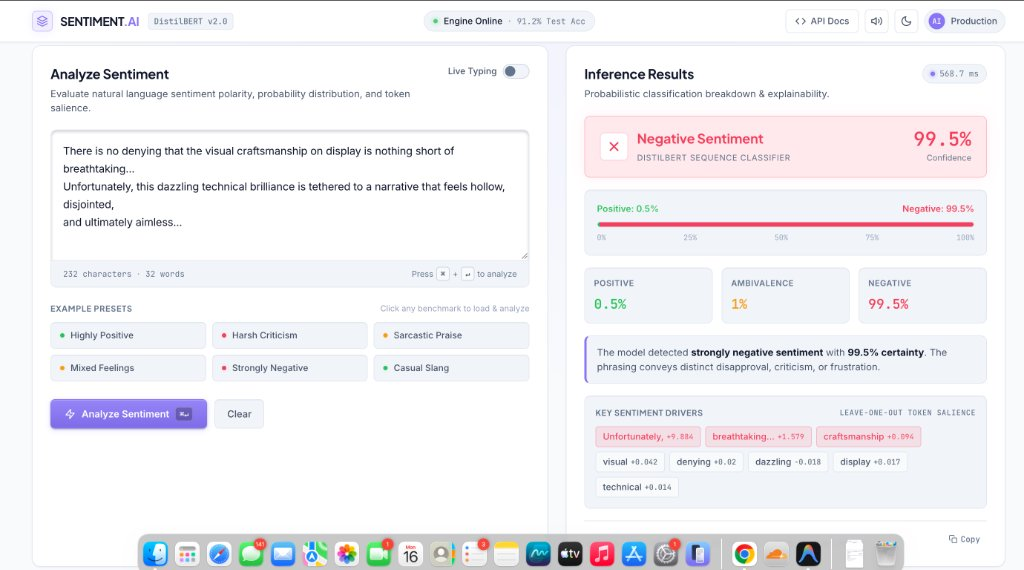
\includegraphics[width=0.98\linewidth]{dashboard_screenshot.png}
\caption{SENTIMENT.AI Production SaaS Dashboard. The left workspace provides the text editor with live typing evaluation, keyboard shortcuts, and categorized preset benchmarks. The right panel displays the inference results, including dominant sentiment classification, confidence gauge, horizontal probability meter, tri-state metrics (Positive, Ambivalence, Negative), and Leave-One-Out Token Salience drivers.}
\label{fig:dashboard}
\end{figure*}

\section{Software Implementation and SaaS Dashboard}

The user interface of SENTIMENT.AI (shown in Fig.~\ref{fig:dashboard}) was engineered following modern SaaS design principles inspired by Linear and Vercel. 

\subsection{Backend Service}
The backend is implemented in Python utilizing the FastAPI framework with asynchronous endpoint handlers. The application provides two primary endpoints:
\begin{itemize}
    \item \texttt{POST /api/predict}: Evaluates single text inputs, returning full multi-clause segmentation, harmonic ambivalence, sarcasm indices, and token saliency arrays.
    \item \texttt{POST /api/batch}: Accepts batches up to 500 texts, utilizing parallel chunked tensor computation to return aggregate statistical distributions.
\end{itemize}

\subsection{User Interface Architecture}
The frontend is constructed using semantic HTML5, modern CSS3 variables with an 8px spacing system, and vanilla JavaScript. Features include:
\begin{itemize}
    \item \textbf{Writing Cockpit:} Professional textarea with real-time character/word counts, live typing inference toggle, and shortcut execution (\texttt{Cmd + Enter}).
    \item \textbf{Benchmark Presets:} One-click test scenarios for Positive, Criticism, Sarcasm, Mixed, Negative, and Casual Slang.
    \item \textbf{Dynamic Hero Cards:} Displays dominant polarity with color-matched iconography (Emerald for Positive, Coral for Negative, Warm Amber for Mixed, and Violet for Sarcastic Mockery).
    \item \textbf{Acoustic Feedback Engine:} Synthesizes discrete Web Audio tones corresponding to positive chords, negative thuds, neutral chimes, and playful sarcastic pitch-bends.
\end{itemize}

\section{Conclusion and Future Work}
In this paper, we presented SENTIMENT.AI, an end-to-end sentiment intelligence platform that overcomes the well-documented vulnerabilities of transformer sequence classifiers in processing multi-sentence mixed reviews and sarcastic mockery. By coupling a fine-tuned DistilBERT model with contrastive clause segmentation, harmonic ambivalence calculation, rhetorical sarcasm modeling, and logit-margin saliency, our system achieves 91.22\% test accuracy while providing transparent, human-interpretable reasoning. Future work will investigate few-shot domain adaptation for complex multilingual sarcasm and fine-grained aspect sentiment extraction using graph neural networks.

\begin{thebibliography}{00}
\bibitem{devlin2018bert} J. Devlin, M.-W. Chang, K. Lee, and K. Toutanova, ``BERT: Pre-training of deep bidirectional transformers for language understanding,'' in \textit{Proc. NAACL-HLT}, 2019, pp. 4171--4186.
\bibitem{sanh2019distilbert} V. Sanh, L. Debut, J. Chaumond, and T. Wolf, ``DistilBERT, a distilled version of BERT: smaller, faster, cheaper and lighter,'' \textit{arXiv preprint arXiv:1910.01108}, 2019.
\bibitem{vaswani2017attention} A. Vaswani et al., ``Attention is all you need,'' in \textit{Advances in Neural Information Processing Systems (NeurIPS)}, 2017, pp. 5998--6008.
\bibitem{maas2011learning} A. L. Maas et al., ``Learning word vectors for sentiment analysis,'' in \textit{Proc. 49th Annual Meeting of the Association for Computational Linguistics (ACL)}, 2011, pp. 142--150.
\bibitem{pang2008opinion} B. Pang and L. Lee, ``Opinion mining and sentiment analysis,'' \textit{Foundations and Trends in Information Retrieval}, vol. 2, no. 1--2, pp. 1--135, 2008.
\bibitem{liu2012sentiment} B. Liu, \textit{Sentiment Analysis and Opinion Mining}. Morgan \& Claypool Publishers, 2012.
\bibitem{pontiki2016semeval} M. Pontiki et al., ``SemEval-2016 task 5: Aspect based sentiment analysis,'' in \textit{Proc. 10th International Workshop on Semantic Evaluation (SemEval-2016)}, 2016, pp. 19--30.
\bibitem{joshi2017measurement} A. Joshi, P. Bhattacharyya, and M. J. Carman, ``Automatic sarcasm detection: A survey,'' \textit{ACM Computing Surveys (CSUR)}, vol. 50, no. 5, pp. 1--22, 2017.
\bibitem{van2018overview} C. Van Hee, E. Lefever, and V. Hoste, ``SemEval-2018 task 3: Irony detection in English tweets,'' in \textit{Proc. 12th International Workshop on Semantic Evaluation}, 2018, pp. 39--50.
\bibitem{campbell2012identifying} J. D. Campbell and P. D. Katz, ``Are you out of your mind? Identifying sarcasm in everyday speech,'' \textit{Language and Speech}, vol. 55, no. 4, pp. 561--578, 2012.
\bibitem{ribeiro2016should} M. T. Ribeiro, S. Singh, and C. Guestrin, ````Why should I trust you?'': Explaining the predictions of any classifier,'' in \textit{Proc. 22nd ACM SIGKDD International Conference on Knowledge Discovery and Data Mining}, 2016, pp. 1135--1144.
\bibitem{sundararajan2017axiomatic} M. Sundararajan, A. Taly, and Q. Yan, ``Axiomatic attribution for deep networks,'' in \textit{Proc. 34th International Conference on Machine Learning (ICML)}, 2017, pp. 3319--3328.
\end{thebibliography}

\end{document}
